\begin{frame}{Experimental Setup}
    Experiments presented in this paper were carried out using the Grid'5000 testbed, supported by a scientific interest group hosted by Inria and including CNRS, RENATER and several Universities as well as other organizations (see https://www.grid5000.fr).\\


    One evaluation on chuc cluster, using 4*A100 40G of VRAM GPU, is taking around 40 minutes. Each algorithms have a budget of 50 evaluations, including the 10 sampling evaluation of BO. 
    
\end{frame}
%---------------------------------- Sampling experiment -------------------------------
\begin{frame}[allowframebreaks]{Sampling experiment : Latin Hypercube Sampling}
    
    \begin{columns}
        \begin{column}{0.45\textwidth}
        Objective : explore the search space and make a reference for other algorithms.
        \begin{block}{Analysis}
            \begin{itemize}
                \item Top scores : \\ \quad Hellaswag : 47.9\% \\ \quad MMLU : 37.6\%
                \item High range for Hellaswag, allowing to discriminate efficiently between solutions.
            \end{itemize}
            
        Running time : arround 36 hours
        
        \end{block}   
    \end{column}

    \begin{column}{0.45\textwidth}
        \begin{figure}
            \centering
            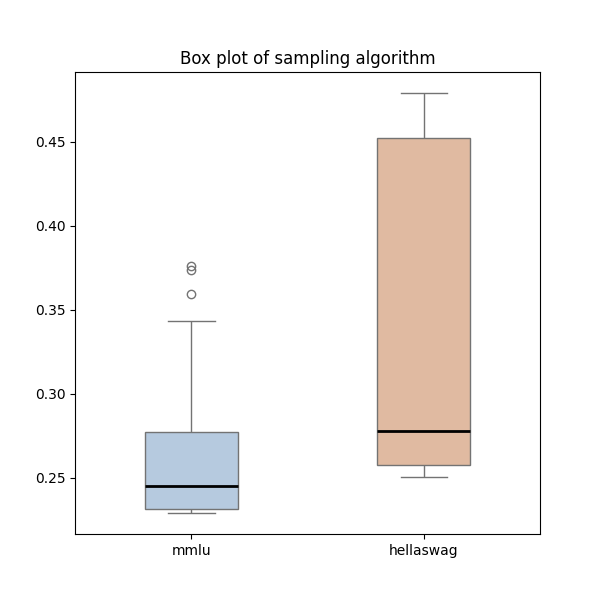
\includegraphics[width = \textwidth]{imgs/experiments/lhs_box_plot.png}     
            \caption{Distribution of score for sampling experiment}         
        \end{figure}
         
    \end{column}
\end{columns}  
    %%%%%%%%%%%%%%%%%%%%%%%%%%%%%%%%%%% BREAK %%%%%%%%%%%%%%%%%%%%%%%%%%%%%%%%%%%
    \framebreak

    \begin{columns}
        \begin{column}{0.3\textwidth}
        \begin{figure}
            \centering
            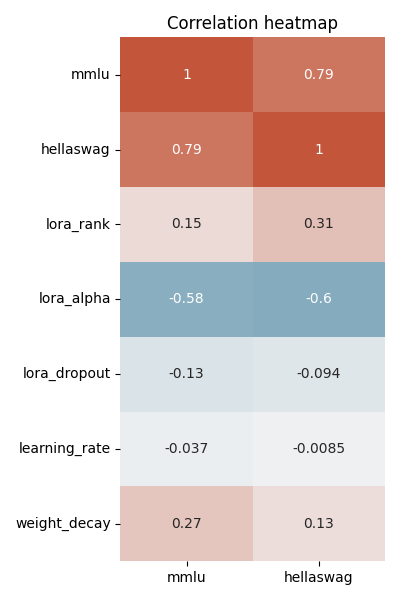
\includegraphics[width = \textwidth]{imgs/experiments/lhs_correlation.png}     
            \caption{Correlation between variables and metrics}         
        \end{figure}
         
        \end{column}
        \begin{column}{0.6\textwidth}
            \begin{block}{Correlation between metrics}
                With 79\% of correlation, Hellaswag and MMLU accuracy are relevant as validation/testing metrics.
            \end{block}
            \begin{block}{Correlation between variables and metrics}
                High factor variables : LoRA alpha the Lora rank / weight decay.\\
                TO DO : verify with other experiment the relevance of using dropout and learning rate.
            \end{block}
        \end{column}
    \end{columns}

\end{frame}



%---------------------------------- Bayesian Optimization -------------------------------
\begin{frame}[allowframebreaks]{BO (waiting for results)}
    
    \begin{columns}
    
        \begin{column}{0.6\textwidth}
            \begin{block}{Score evolution}
                \begin{figure}
                    \centering
                    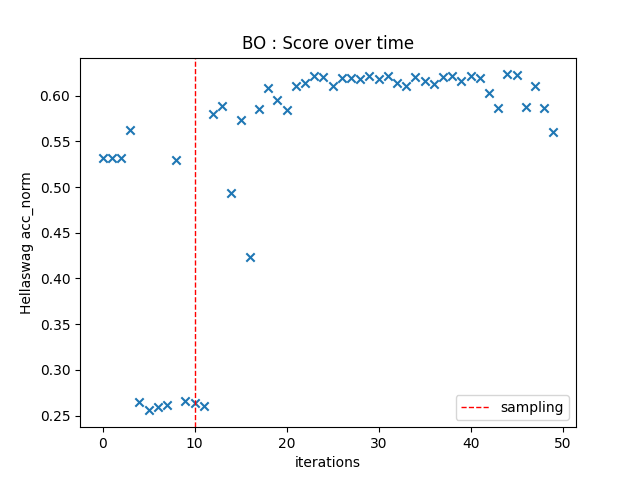
\includegraphics[width = 7.5cm]{imgs/plots/exp12_score_over_time.png}
                    \caption{Score over time}
                \end{figure}
            
            \end{block}   
        \end{column}

        \begin{column}{0.4\textwidth}
            \begin{block}{Results}
                Best score : 62.3\%, achieved after X iterations. \\   
                Wait for MMLU to look at overfitting            
            \end{block}

            \begin{block}{Behavior}
                \begin{itemize}
                    \item 0 -> 10 : sampling (LHS)
                    \item 10 -> 25 : converge to high score
                    \item 25 -> 40 : high score
                    \item 40 -> 50 : search unexplored space
                \end{itemize}
                
            \end{block}
             
        \end{column}
    \end{columns}    

    %%%%%%%%%%%%%%%%%%%%%%%%%%%%%%%%%%% BREAK %%%%%%%%%%%%%%%%%%%%%%%%%%%%%%%%%%%
    \framebreak

    \begin{columns}
    
        \begin{column}{0.65\textwidth}
            \begin{block}{Exploitation of the search space}
                rank, alpha and learning rate seem to converge fast\\
                weight decay converge slowly to the top during high score phase\\
                
                dropout does not converge, linked with weak correlation to metrics => relevant Hyperparameter ?? 
            \end{block}
        \end{column}

        \begin{column}{0.35\textwidth}
            \begin{figure}
                \centering
                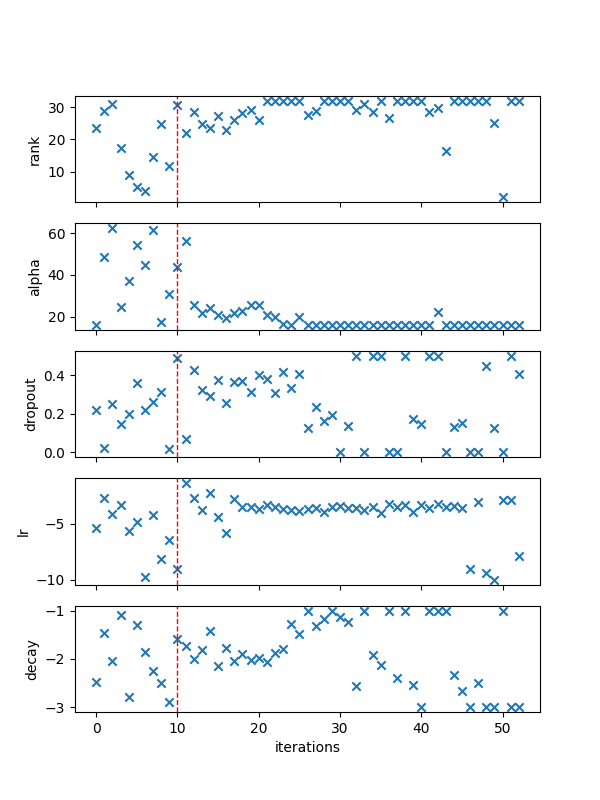
\includegraphics[width = \textwidth]{imgs/plots/exp12_variables_over_time.png}
                \caption{Variables over time}
            \end{figure}
            
            
        \end{column}
    \end{columns}  
\end{frame}

%---------------------------------- Optimization -------------------------------
\begin{frame}[allowframebreaks]{SOO(waiting for results)}
    
    \begin{columns}
    
        \begin{column}[t]{0.6\textwidth}
            \begin{block}{Score evolution}
                
                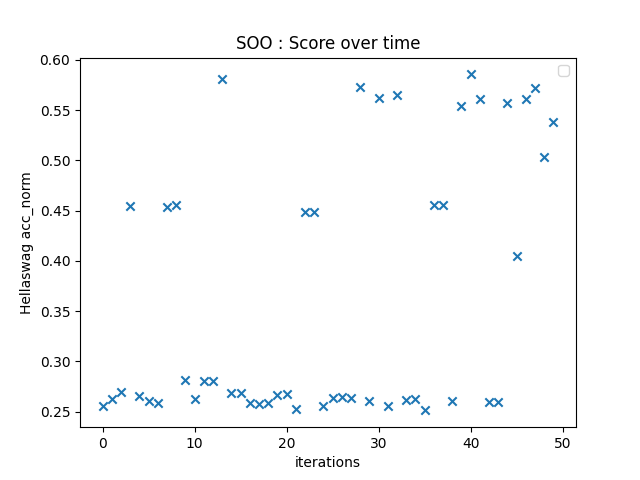
\includegraphics[width = 7.5cm]{imgs/plots/exp10_score_over_time.png}
            
            \end{block}   
        \end{column}

        \begin{column}[t]{0.4\textwidth}
            \begin{block}{Results}
                Best score : 58.4\%\\              
            \end{block}

            \begin{block}{Behavior}
                Slow convergence, need more than 50 iterations to converge to more depth. 
                Max depth : 6
                A lot of unpromising point to explore
                
            \end{block}
            
            
        \end{column}
    \end{columns}   
    
    \framebreak

    \begin{columns}
    
        \begin{column}{0.65\textwidth}
            \textbf{Score by variables and Varibles over iterations}
                \begin{figure}[h]
                    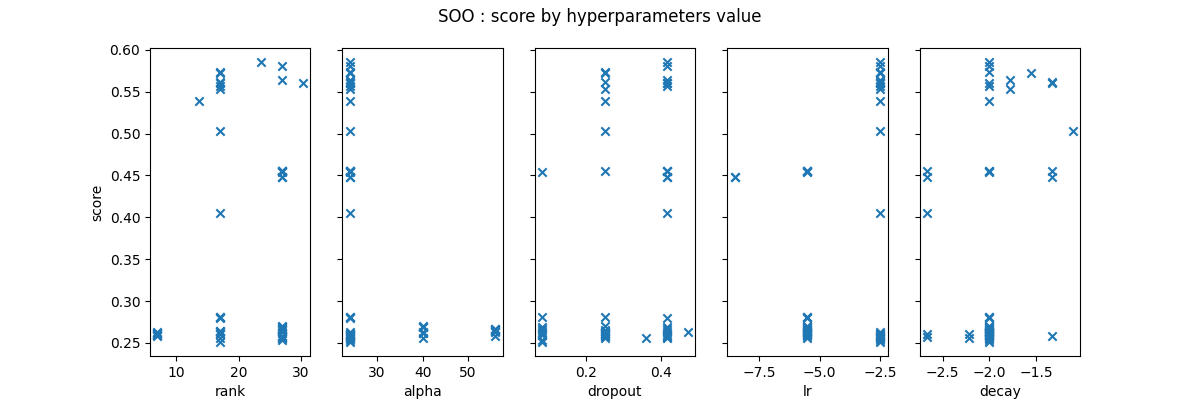
\includegraphics[width = \textwidth]{imgs/plots/exp10_score_by_hp.png}
                \end{figure}     
        \end{column}

        \begin{column}{0.4\textwidth}
            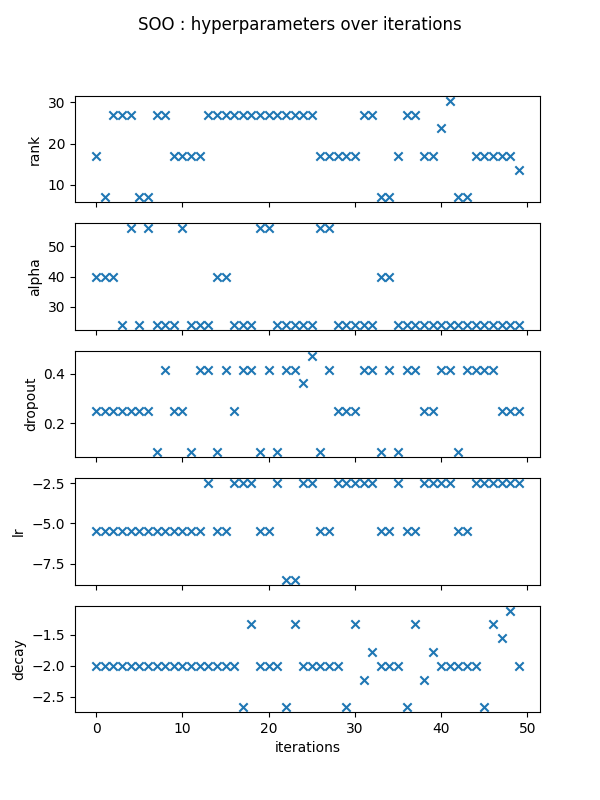
\includegraphics[height = 7cm]{imgs/plots/exp10_variables_over_time.png}
            
            
        \end{column}
    \end{columns}  
\end{frame}

%---------------------------------- Optimization -------------------------------
\begin{frame}[allowframebreaks]{BaMSOO}
    
    \begin{columns}
    
        \begin{column}[t]{0.6\textwidth}
            \begin{block}{Score evolution}
                
                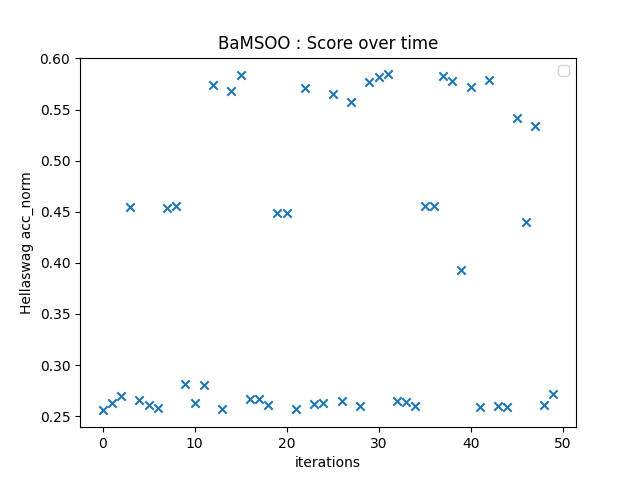
\includegraphics[width = 7.5cm]{imgs/plots/exp11_score_over_time.png}
            
            \end{block}   
        \end{column}

        \begin{column}[t]{0.4\textwidth}
            \begin{block}{Results}
                Best score : 58.5\%\\
                Not so much approximations, need to increase $\eta $ in equation \ref{eq:ucb} to speed the convergence              
            \end{block}
            
            
        \end{column}
    \end{columns}    

    \framebreak

    \begin{columns}
    
        \begin{column}{0.65\textwidth}
            \textbf{Score by variables and Varibles over iterations}
                \begin{figure}[h]
                    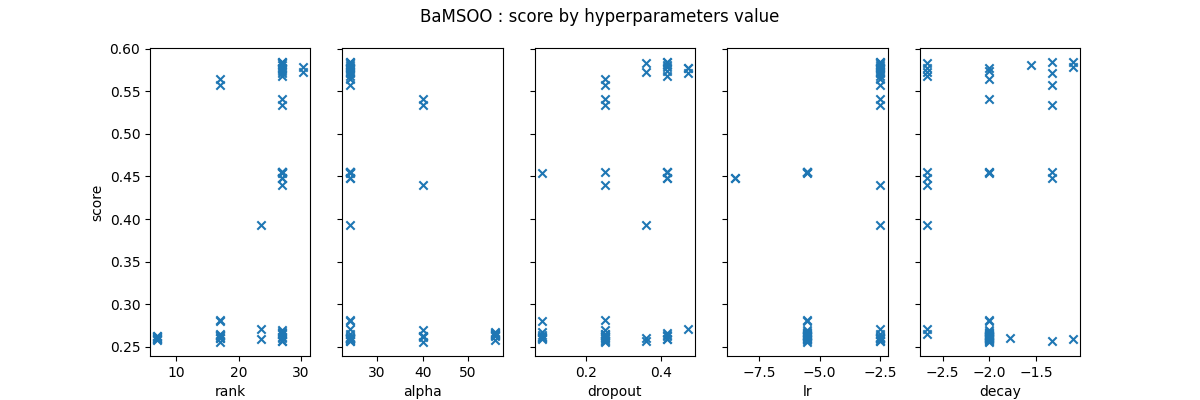
\includegraphics[width = \textwidth]{imgs/plots/exp11_score_by_hp.png}
                \end{figure}     
        \end{column}

        \begin{column}{0.4\textwidth}
            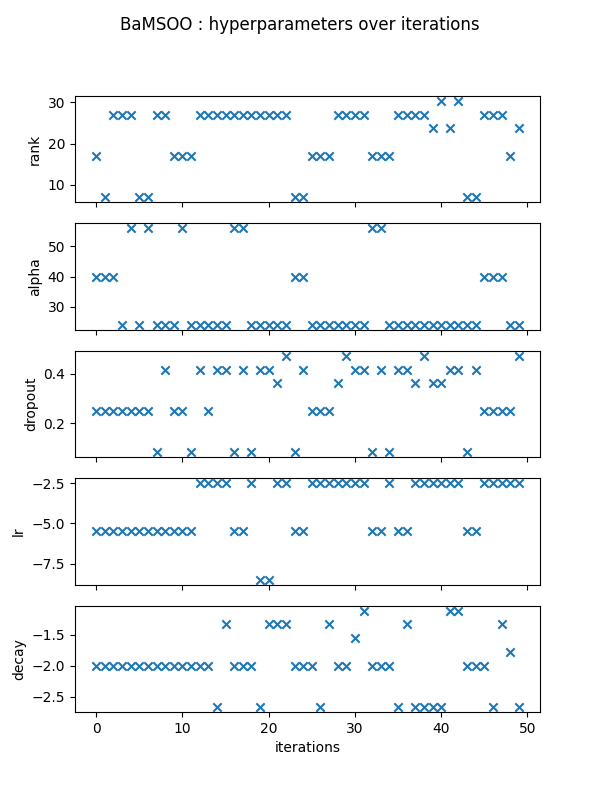
\includegraphics[height = 7cm]{imgs/plots/exp11_variables_over_time.png}
            
            
        \end{column}
    \end{columns}  
\end{frame}

%%%%%%%%%%%%%%% COMPARISON %%%%%%%%%%%%%%
\begin{frame}{Comparison (waiting results)}

    \begin{table}[ht!]
        \centering
        \begin{tabular}{|c||c|c||c|c|c|}
        \hline
           Datasets  & Lower (LHS) & Upper & BO & SOO & BaMSOO \\
        \hline
           Hellaswag  & 47.9 & 69.8* & X & X & X \\
           MMLU & 37.6 & 49.3 & X & X & X  \\
        \hline
        \end{tabular}
        \caption{Bounds on accuracy for validation and testing dataset}
        \label{tab:bounds}
    \end{table}

\end{frame}